\chapter{\etherbase: Improving Reproducibility in Smart Contract Research} \label{ch:etherbase}


\textit{
	This chapter is adapted from work supervised by Jeremy Clark and Amir G. Aghdam, to-be-submitted at the 7th Workshop on Trusted Smart Contracts (WTSC) co-located with Financial Cryptography and Data Security (FC).
}

\section{Introductory Remarks}
	\label{sec:intro}
	Ethereum blockchain handles financial assets and contracts with millions of USD in value.
	It is the most widely used blockchain platform with millions of smart contracts written on it.
	A smart contract is simply a program stored on the Ethereum blockchain that runs when predetermined conditions are met.
	There has been some effort from the research community to develop automated analysis tools and frameorks~\cite{ref_tools} that locate and eliminate vulnerabilities in smart contracts.
	These tools and frameworks analyze smart contracts and produce vulnerability reports.
	In a preliminary study performed on nearly one million Ethereum smart contracts, using one analysis framework for verifying correctness, the researchers flagged 34,200 of them as vulnerable.~\cite{ref_flag1}
	A different study showed that of 19,366 smart contracts analysed, also in Ethereum, 8,833 (around \%46) were flagged as vulnerable.~\cite{ref_flag2}

	Famous attacks, such as The DAO exploit~\cite{dao} and the Parity wallet bug~\cite{ref_parity} illustrate this problem and have led to substantial financial losses and consequent effort from the research community to counter such incidents.

	However, it is not easy to compare and reproduce such research; even though several of the tools built by the research community are publicly available, the datasets used to test and benchmark those very same tools are not.

	If the developer of a new tool intends to compare their new tool with existing work and projects, the current approach is to contact the authors of alternative tools and hope for access to the same datasets or make do with whatever out-of-date incomprehensive and unrepresentative dataset they have at their disposal, a very timely and inefficient process.

	In other cases, the researchers need to start from scratch and create their own datasets, a non-trivial and slow process.
	What makes it worse is the data bias, which can be introduced in a dataset in different phases of data acquisition and data cleaning.
	This can easily escalate to become a threat to validity in the research.~\cite{Empirical-Evaluation-of-Smart-Contract-Testing:What-is-the-Best-Choice}

	In this chapter, we present \etherbase, an extensible, queryable, and easy-to-use database that facilitates and enhances the verification and reproducibility of previous empirical research and lays the groundwork for faster, more rapid production of research on smart contracts.
	\etherbase is open-source and publicly available online at: \textbf{link TBD}.
	The source code for data acquisiton and cleaning is not available due to private IP reasons, and only the collected data and the database is accessibel to the public.
	Researchers, smart contract developers, and blockchain-centric teams and enterprises can also use such corpus for specific use-cases.

	We also note that although \etherbase has been implemented for Ethereum, it can be easily extended to support other blockchains which have the similar design for smart contracts with Ethereum.

	In summary, we make the following contributions with \etherbase.
	\begin{enumerate}
		\item We propose \etherbase, a systemic and up-to-date database for Ethereum by exploiting its intetrnal mechanisms.
		\item We implement \etherbase after addressing several technical challenges. It obtains historical data and enables new functionalities. It is more up-to-date than existing datasets, gets systematically reviewed and renewed, in comparison to the previous manual one-time data gathering efforts.
		\item We propose the first dataset of Ethereum smart contracts which has a mix of off-chain and on-chain data together, meaning that it contains the source code and the bytecode of the corresponding smart contracts in the same dataset.
		\item We propose the first automatically up-to-date laballed dataset of Ethereum smart contracts with vulnrabilities.
	\end{enumerate}

\section{Related Work}
	\label{sec:relwork}
	We assume the reader is familiar with blockchain technology, Ethereum blockchain, and its primary high-level programming language Solidity.
	Ethereum Smart contracts written in Solidity are compiled to bytecode to be executed on the Ethereum Virtual Machine (EVM).
	EVM takes bytecode as input and works in a stack-based architecture with a word size of 256 bits.
	There are three different spaces in EVM to store data and resources, namely stack, memory and storage.
	In this section we present and discuss references and information for some of the more prominent publicly available smart contract benchamrk datasets which were identified in our studies.

	SmartBugs~\cite{Empirical-Review-of-Automated-Analysis-Tools-on-47587-Ethereum-Smart-Contracts} makes the top of the list as one of the most used benchmarks in the research space.
	Durieux et al. crafted a dataset of annotated and non-annotated smart contracts.
	The annotated part contains 69 contracts tagged with 115 vulnerabilities.
	The annotated part has ten categories of vulnerabilities.
	In contrast, the non annotated part contains 47,518 unique contracts, each with at least one transaction on the Ethereum network.
	Researchers can't use the unlabeled dataset to evaluate the tool as there is no ground truth associated with it.
	Moreover, the labeled dataset doesn't have more than a thousand smart contracts and only the source code (and no bytecode) of the contracts are available.

	Ren et al.~\cite{Empirical-Evaluation-of-Smart-Contract-Testing:What-is-the-Best-Choice} crafted a benchmark suite that integrates labeled and unlabeled Smart Contracts from a variety of sources such as Etherscan~\cite{etherscan}, SolidiFI repository, Common Vulnerabilities and Exposures Library, and Smart Contract Weakness Classification and Test Cases library.
	The unlabeled dataset has 45,622 Real-World Ethereum Smart Contracts having more than one transaction on the Ethereum blockchain.
	The labeled dataset has artificially constructed contracts (350 contracts) and confirmed vulnerable contracts (214 contracts).

	Many vulnerability analysis tools used unlabelled datasets to evaluate the tool.
	Due to huge number of contracts in these datasets, either the dataset is not annotated or a very small subset is annotated with the vulnerabilities present.
	To the best of our knowledge, there is no fully annotated dataset released publicly.

	Kalra et al.~\cite{kalra2018zeus} published their analysis results for 1,524 smart contracts with no other information or metadata in relation to those contracts.

	Luu et al.~\cite{oyente} collected 19,366 smart contracts from the blockchain and provided their blockchain addresses alongside analysis results on each contract on whether they contain any of their selected four vulnerabilitis or not.

	The smart contract source codes collected in GitHub typically do not directly reference smart contracts deployed on the blockchain through an Ethereum address;
	therefore, it is hard to determine whether it has been tested or used on the blockchain or not.
	GitHub repositories of the available datasets do not implement a search engine or query capability to filter smart contracts based on particular metrics or parameters, such as the ETH value or the number of internal transactions for a smart contract.
	On a GitHub repository, there is no information on smart contracts' use in a real blockchain scenario, on the number of transactions invoking smart contracts or on the number of tokens associated with each smart contract.
	None of the GitHub repositories currently available to the public or used in research papers provide smart contract ABI's or Opcodes to the best of our knowledge.
	
	Concerning the block explorer Etherscan, they allow for exploration and search of Ethereum blockchain for smart contracts.
	However, when downloading the smart contracts' source code, the block explorer presents some limitations: 
	Smart contracts' data and numbers in quantity are massive (on the Giga scale, based on our estimation), but there is a limited API rate of 100 submissions per day per user to retrieve just a smart contract, making the complete download of data an impossible endeavour.
	Etherscan's API does not provide facilities to obtain a list of the smart contracts' addresses, as the existing API calls mainly allow navigation from one block to another.
	A researcher cannot directly and easily explore the smart contracts' source code but has first to inspect any block in Ethereum and then look for all the transactions that involve an address associated with the smart contract.

\section{Methodology}

	\begin{figure}[t]
		\centering
		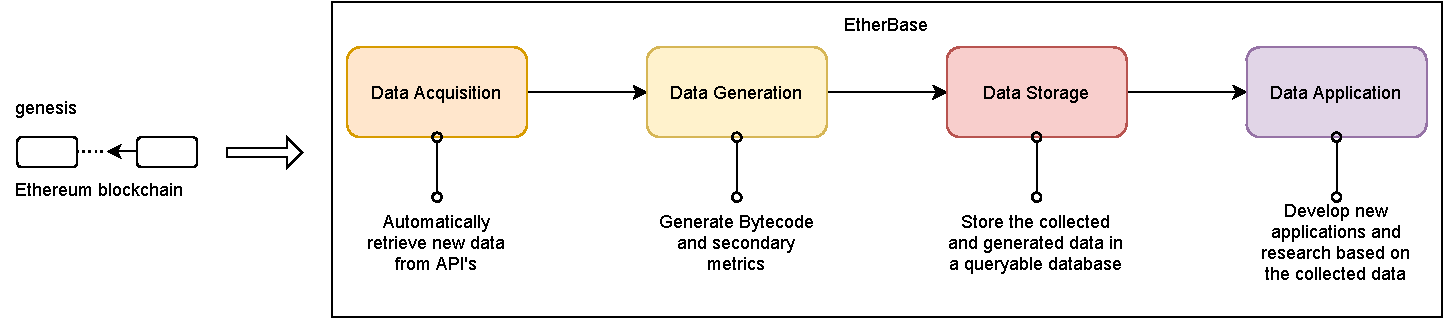
\includegraphics[width=1\textwidth]{figures/Untitled Diagram.pdf}
		\caption{EtherBase Worflow}
		\label{fig:my_label}
	\end{figure}
	
	We specifically designed \etherbase to not provide the end-users with a dump of contracts and their corresponding features in a vague file hierarchy.
	We have a service offering the ability to filter and analyze smart contracts and a dataset of smart contracts with interesting features to conduct empirical research on, according to metrics like Pragma version, ETH value, etc.
	To fulfill its purpose, \etherbase is designed to perform four primary automatic operations on the data:
	\begin{enumerate}
		\item \textbf{Data Acquisiton}: Automatic retrieval of off-chain and on-chain data
		\item \textbf{Data Generation}: Generation of bytecode and other metrics
		\item \textbf{Data Storage}: Storage of the collected data in a public and accessible way
		\item \textbf{Data Application}: Development of new applications and research based on the available database
	\end{enumerate}

	The next sections walk through the above-mentioned steps of the workflow one-by one.

	\subsection{Data Acquisition}
		The current dataset is collected from Etherscan, which is the largest decentralized platform for Ethereum smart contracts.
		All contracts stored on Etherscan are indexed by unique addresses, so we first retrieve the addresses of all contracts that have more than one transaction through Google BigQuery.
		Using Google BigQuery query request service, we obtain 1,712,347 distinct contract addresses that have more than one transactions associated with them.

	\subsection{Data Generation}
		Instead of writing scripts to obtain the bytecode and/or source code thrpugh Etherscan's API, we leverage a tool designed and maintained by Trail of Bits, namely Cyitic-compile.
		All the previous works of research, work on providing either source code or bytecode of smart contracts to the researchers, but that will not be enough for the users who want to compile the smart contracts or build tools upon such data.
		Compiling smart contracts is also a tricky busines, due to the rapid pace of changing versions of the dominant programming language, Solidity, used to write and develop smart contracts.
		We developed crytic-compile, a library to help the compilation of smart contracts, to help with this problem.
		It helps the user to be needless of maintaining an interface with solc and it automatically finds and uses the right version of solc or a better compatiable version of solc to compile the input smart contracts.
		They way this works under the hood is that crytic-compile compiles an input smart contract and outputs a compilation untit in the standard solc output format, written in a json file, alongside the source code and other metadata.
		Unlike the other proposed datasets and tools discussed in Section~\ref{sec:relwork}, EtherBase targets the core problem of the lack of reproducibility in the research literature.
		Discussions surrounding what types of secondary metrics to retrieve from the Ethereum blockchain or third-party services will be explored further.
		For further analysis, we only retain source-available contracts.
		Then we adopt the method used in~\cite{deduplicate} to remove the duplicates, that is checking whether the MD5 checksums of the two source files are identical after removing all the blank lines and comments.
		After deduplication, we get 48,622 unique contracts.
		For this paper and as of now, we have released 5,000 smart contracts for the tool comparison purposes in \etherbase~due to the technical challenges given in Section~\ref{section:challenges}.
		There exist many metrics that we have access to, can calculate, and add to \etherbase, but not a lot of research has been conducted on the applicability of these many different types of metrics to empirical research on the Ethereum blockchain or how much it appeals to the researchers active in this field.
		In the following, we describe the initial set of the metrics we selected to include in EtherBase in the form of a table, to be followed by more, after more discussion and research on their applicability to research on smart contracts.

		The built-in metrics relating to smart contracts are those features which depend on the internal properties of a smart contract, e.g. SLOC (Source Lines of Code), Pragma version, number of modifiers, payable, etc. Hence the title \emph{primary metrics}.

		For this table, we decided to include the core metrics of a smart contract, which would help a researcher collect a large set of smart contracts rapidly, and conduct further analysis on them, comprising of:

		\begin{table}[H]
			\caption{Primary Metrics on Smart Contracts}
			\label{tab:intrinsic-cues}
			\centering
			\begin{adjustbox}{width=1\textwidth}
			\def\arraystretch{1.3}
			\begin{tabular}{l|p{105mm}}
				\textbf{Name} & \textbf{Description} \\
				\hline
				\verb|Pragma| & The \verb|pragma| keyword is used to enable certain compiler features or checks.\\
				\verb|Contract Address| & Unique 20-byte address, used as the main index to distinguish smart contracts from each other. \\
				\verb|Creator Address| & Indicates the address of the deeployer of the smart contract. \\
				\verb|Source Code| & Source code of the smart contract, specific to the programming language Solidity. \\
				\verb|Bytecode (bin)| & . \\
				\verb|Bytcode (bin-runtime)| & . \\
				\verb|ABI| & The content of the application binary interface for each contract. \\
				\verb|Block Number| & The length of the blockchain in blocks. \\
				\verb|ETH Value| & The value of each smart contract in therms f=of the ETH thay hold. \\
				\verb|Transaction Count| & Number of internal transactions from eacch smart contract. \\
				%\verb|Deployer Status| & Indicates whether the deployer of a contract is a contract or not. \\
			\end{tabular}
			\end{adjustbox}
	\end{table}

	As for the primary metrics, here are our justifications for the above selection:

	\begin{itemize}

		\item{\verb|Pragma|: Source files can (and should) be annotated with a version pragma to reject compilation with future compiler versions that might introduce incompatible changes. Filtering through contracts via Pragma helps the researcher to collect a homogenuous set of contracts with a consistent synatx.}\\

		\item{\verb|Contract Address|: In Ethereum, the state is made up of objects called "accounts", with each account having a 20-byte address. Contract address is the main key in EtherBase for distinguishing contracts from each other.}\\

		\item{\verb|Creator Address|: The contract address is usually given when a contract is deployed to the Ethereum Blockchain. The address comes from the creator's address, where the contract has been initially deployed from, alongside the number of transactions sent from that address (the “nonce”). A creator's address can be helpful in analyzing the clone ratio and }\\

		\item{\verb|Source Code|: The source code of each Ethereum smart contract is written in Solidity and helps researchers do all sortds of analysis on the smart contracts.}\\

		\item{\verb|Bytecode (bin)|: The regular \verb|bin| output is the code placed on the blockchain plus the code needed to get this code placed on the blockchain, the code of the constructor.}\\

		\item{\verb|Bytecode (bin-runtime)|: \verb|bin-runtime| is the code that is actually placed on the blockchain.}\\

		\item{\verb|ABI|: \verb|ABI| stands for application binary interface. It's basically how you can encode Solidity contract calls for the EVM and, backwards, how to read the data out of transactions.}\\

		\item{\verb|Block Number|: \verb|Block Number|is the length of the blockchain in blocks, more specifically the block on which the smartt contract exists.}\\
		\item \verb|ETH Value|: The ETH every smart contract hols is an excellent filter or bar to select "interesting" contracts through for further research on the contracts that are more \emph{active} on the blockchain.\\

		\item \verb|Transaction Count|: Like ETH Value, transaction count is an important metric for us to be able to exclude contracts that do not participate much on the chain and hence, work on the contracts thast have a higher probability of interaction with more contracts.\\
		\end{itemize}
	
		\subsection{Data Storage}
			In the data storage stage, all extracted data are stored in PostgreSQL-alongside a GitHub repository- for the ease of data management.
			Users can get access to the collected data in PostgreSQL.
			In the application stage, users can conduct various analyses on the collected data.

			Figure 2 shows the directory structure of the collected data. The first leaf in the directory \texttt{Contracts} corresponds to the \\


\definecolor{folderbg}{RGB}{124,166,198}
\definecolor{folderborder}{RGB}{110,144,169}

\def\Size{4pt}
\tikzset{
  folder/.pic={
    \filldraw[draw=folderborder,top color=folderbg!50,bottom color=folderbg]
      (-1.05*\Size,0.2\Size+5pt) rectangle ++(.75*\Size,-0.2\Size-5pt);  
    \filldraw[draw=folderborder,top color=folderbg!50,bottom color=folderbg]
      (-1.15*\Size,-\Size) rectangle (1.15*\Size,\Size);
  }
}
\resizebox{0.6\textwidth}{!}{%
\begin{forest}
  for tree={
    font=\ttfamily,
    grow'=0,
    child anchor=west,
    parent anchor=south,
    anchor=west,
    calign=first,
    inner xsep=7pt,
    edge path={
      \noexpand\path [draw, \forestoption{edge}]
      (!u.south west) +(7.5pt,0) |- (.child anchor) pic {folder} \forestoption{edge label};
    },
    before typesetting nodes={
      if n=1
        {insert before={[,phantom]}}
        {}
    },
    fit=band,
    before computing xy={l=15pt},
  }  
[contracts
  [0
  ]
  [1
    [0
      [0
        [0
          [0
            [5
              [0x100005bc082d49eefffdc720864984bd7f3f7e5e
                [0x100005bc082d49eefffdc720864984bd7f3f7e5e-SudEX.sol
                ]
                [artifact.zip
                ]
                [slither-findings.json
                ]
                [slither-findings.md
                ]
                [slither-findings.txt
                ]
              ]
            ]
          ]
          [...
          ]
          [f
          ]
        ]
        [...
        ]
        [f
        ]
      ]
      [...
      ]
      [f
      ]
    ]
    [...
    ]
    [f
    ]
  ]
  [...
  ]
  [f
  ]
]
\end{forest}
}%
\newline
The \texttt{artifact.zip} file contains

\resizebox{0.3\textwidth}{!}{%
\begin{forest}
  for tree={
    font=\ttfamily,
    grow'=0,
    child anchor=west,
    parent anchor=south,
    anchor=west,
    calign=first,
    edge path={
      \noexpand\path [draw, \forestoption{edge}]
      (!u.south west) +(7.5pt,0) |- node[fill,inner sep=1.25pt] {} (.child anchor)\forestoption{edge label};
    },
    before typesetting nodes={
      if n=1
        {insert before={[,phantom]}}
        {}
    },
    fit=band,
    before computing xy={l=15pt},
  }
[\texttt{objects}
  [\texttt{compilation\_units}
    [contract.sol
        [compiler]
        [asts]
        [contracts
            [contracts.sol
                [abi]
                [bin]
                [bin-runtime]
                [srcmap]
                [srcmap-runtime]
            ]
            [SafeMath]
            [...]
        ]
    ]
  ]
]
\end{forest}
}%

	In addition to making the datasets available on GitHub, \etherbase also enjoy a graphical user interface (GUI) in order to allow the less technical end users access and browse through the database.
	We integrated \etherbase with Apache Superset, a powerful business intelligence tool, which lets you creata charts and dashboards using the data from the database.

\subsection{Data Application}
	In order to showcase an application of the empirical usage of the data from \etherbase,  the 5,000 filtered smart contract data set is labelled using three of the most prominently used static analysis tools in Ethereum research that detect various vulnerabilities in smart contracts, using a majority voting mechanism, in order to see how they fare against each other based an automatically labelled dataset.
	The criteria we used for tool selection was pretty simple; we wanted tools that had a focus on assessing Solidity source code instead of bytecode, and that they are available as open-source software and can be evaluated based on their vulnreability detection mechanisms.
	Based on such criteria, we selected the following three tools for our Data Application phase experiment:
	\begin{itemize}
		\item \textbf{Slither:} Slither~\cite{slither} is a static analysis tool designed to analyze Ethereum smart contracts. It has four prominent use cases: automated detection of vulnerabilities, automated detection of code optimization opportunities, improvement of users' understanding of the contracts, and assistant with code review.
		\item \textbf{Mythril:} Mythril is a tool that does security analysis of Ethereum smart contracts. It detects various security issues~\cite{mythril}.
		\item \textbf{Smartcheck:} Smartcheck~\cite{smartcheck} is an extensible static analysis tool that detects vulnerabilities in smart contracts. It converts Solidity code into XML-based intermediate representation and checks it with XPATH patterns.
	\end{itemize}
	
	
	We select three of the highest ranked vulnerabilities according to the DASP 10 ranking by the NCC Group, to test the aforementioned tools based upon.
	The thre vulnerabilities, as explained in Chapter 2, are as follows:
	\begin{itemize}
		\item \textbf{Re-entrancy} also known as the recursive call vulnerability, with SWCRegistry ID SWC-107.
		\item \textbf{Arithemtic:} concerning the integer overflows and underflow vulnerabilities in smart contracts, with SWCRegistry ID SWC-101.
		\item \textbf{Unchecked Ether:} also known as or related to silent failing sends, which can lead to unexpected behavior if return values are not handled properly, with SWCRegistry ID SWC-104.
	\end{itemize} 
	
	\begin{table}[t]
		\caption{Supported Vulnerabilities}
		\label{tab:freq}
	   %\renewcommand{\arraystretch}{1.2}
		\begin{tabular}{cccc}
	  
	  \multirow{2}{*}{\textbf{Tool Name}} & \multicolumn{3}{c}{\textbf{Vulnerability Type}} \\
		 & ARTHM & RENT & UE \\ \midrule
		  Slither    & \crossmark  &  \checkmark  &  \checkmark  \\
		  Mythril    & \checkmark  &  \checkmark  &  \checkmark  \\
		  Smartcheck & \checkmark  &  \crossmark  &  \checkmark  \\
		  \bottomrule
	  \end{tabular}
	  \label{table:vuln_supported_per_tool}
	  \end{table}
	
	
	%Table \ref{table:vuln_supported_per_tool} shows these vulnerabilities supported by the selected tools.
	The \checkmark symbol shows that the tool can detect a particular vulnerability, whereas symbol \crossmark indicates that the tool can't detect the vulnerability.
	
	We use the methodology given in the paper by Ren et al.~\cite{Making-Smart-Contract-Development-More-Secure-and-Easier} to detect the selected vulnerabilities in smart contracts.
	
	Because of the presence of false positives in the reports generated by the static analysis tools, we cannot depend on just one of them.
	We use majority voting, that is, at least 50\% of the tools must report the same vulnerability at the same location.
	For example, assume that tools T1, T2, and T3 can detect the re-entrancy vulnerability.
	Suppose, at least two tools report that vulnerability is present in a smart contract in test.
	Then we say that the contract is vulnerable;
	Otherwise, we say that the contract is not vulnerable.
	
	The following steps explain the methodology given the majority voting mechanism explained above:
	
	\begin{enumerate}
	
	\item First, collect the output of the selected tools for the smart contract to be analyzed.
	
	\item Note the vulnerability name and line number for the vulnerability per tool. 
	
	\item For the same vulnerability, if different tools show different locations, consider them as different warnings. We consider two warnings as the same only if the vulnerability name and location match for different tools.
	
	\item The methodology says that the vulnerability exists at a location if more than 50\% of the tools (2 out of 3 in this experiment scenario) confirm the same vulnerability at the exact location. In that case, label the location with the vulnerability.
	
	\end{enumerate}
	
	\begin{figure}[t]
		\centering
		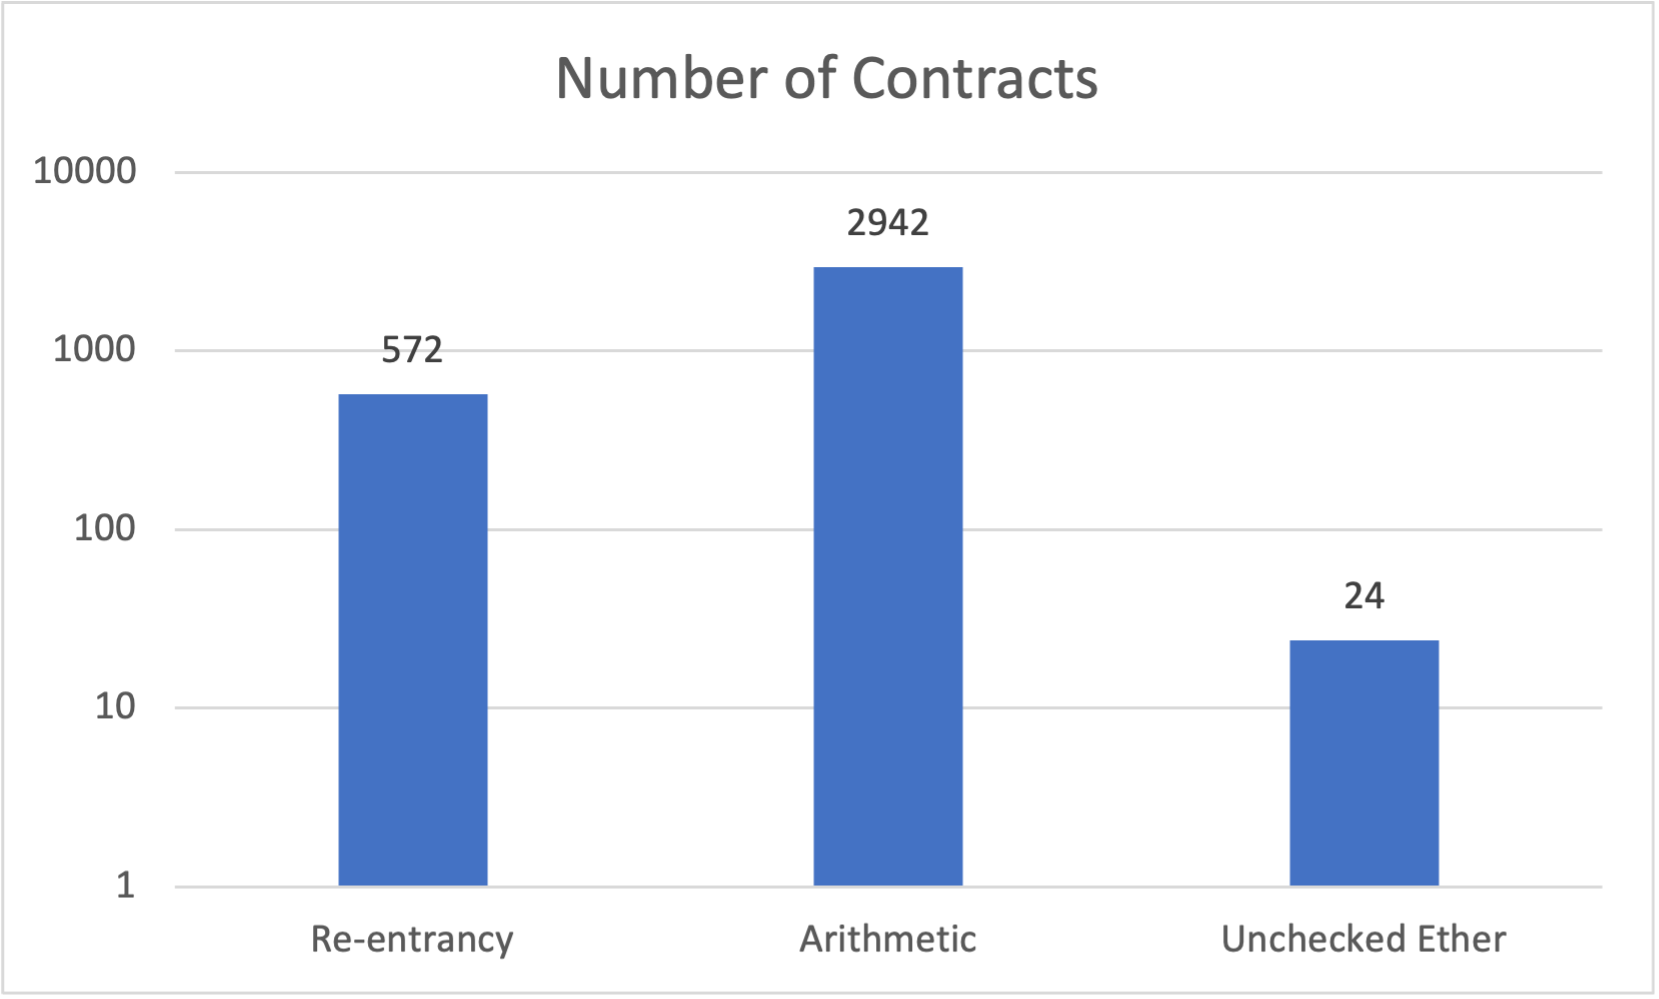
\includegraphics[width=1\textwidth]{figures/Picture1.png}
		\caption{No. of Contracts containing vulnerabilities (log-scale)}
		\label{fig:chart_vuln_count}
	\end{figure}
		
		Figure~\ref{fig:chart_vuln_count} shows the number of smart contracts that contain at least one vulnerability.
		For instance, consider the Re-entrancy vulnerability.
		The literature tells us that all fo the the three static analyzers in the benchmark support the detection of this vulnerability.
		We say that the contract contains reentrancy only if two of these three tools report that it is present at the same location.


\section{Concluding Remarks}
	This chapter introduces an up-to-date database, centred around Ethereum smart contracts, namely \etherbase, which includes data on the Ethereum blockchain (blocks), its smart contracts, and their metadata.
	Moreover, aggregate statistics and dataset exploration is presented.
	Furthermore, future research directions and opportunities are outlined:

	During the time we were building EtherBase, we utilized Web3 APIs without taking advantage of an Ethereum full / archive node.
	The next version of \etherbase we're already working on, will take full use of an Ethereum full node and instrment it in order to add a variety of more data to EtherBase.
	Collecting data via invoking Web3 API's is very much slower than instrumenting an Ethereum archive node.
	
	In addition, our current method is restricted by the rate limit imposed by the API's.
	For example, Etherescan restricts the frequency of invoking its API to 5 queries per second. We plan to solve this as well to speed the automated processes.

	We will also be labelling more smart contracts with more tools as we have more time and compute resources moving forward.

	The Ethereum security research community can use \etherbase for evaluating correctness and other parameters of their proposed or other toolsets, especially those based on machine learning techniques that need comprhensiver datasets for training, validation, and testing phases.
	\etherbase~comprises a diverse and comprehensive set of real-world heterogenuous annotated smart contracts.
	
	Every tool which was selected for this evaluation is not a complete one.
	There are always many false positive / negatives results generated by a static analyser.
	Nevertheless, we utilized the mechanism of majority voting to determine the presence or lacke of precense of a vulnerability in a smart contract.
	But, this approach may fail if majority of the tools generate false positives or false negatives.
	Such issues can be overcome by adding more tools to the benchamrk process or have some auditors manually review the discovered potential vulnerabilities..
	However, these approaches are time and resource-intensive, and we can plant to implement it incrementally.